\subsection{Authorization Components}
The authorization components are designed to provide access control: to build
and maintain a set of eligible voters, administrators, and whatever other roles
might be necessary to implement the electoral systems. Ultimately, the
authorization components are responsible for restricting access to sensitive
contract function calls that mutate the state of the contract, e.g., casting
ballots and configuration elections. The design must be flexible enough to
facilitate the varying and evolving needs of different organizations and
communities but consistent enough to support them all through a common
interface. Concepts are borrowed from traditional operating system access
control schemes/models and authorization mechanisms which provide guidance for
system design. The underlying authentication features are handled via the
asymmetric cryptography provided by the underlying blockchain infrastructure.

\subsubsection{Access Control}
Access control schemes exist to authorize access to data and resources; they are
responsible for managing and defining the relationships between permissions,
operations, objects, and subjects. Several access control model schemes were
considered in this phase; among them were: access control lists, discretionary
access control, mandatory access control, and role-based access control.

\paragraph{Discretionary Access Control}
Discretionary Access Control (DAC) is a form of access control where the owner
of some resource/object can dictate the operations and permissions that other
subjects can take on the resource/object. Additionally, the owner of the
resource/object can pass ownership to some other subject. You can see a form of
this in POSIX file systems where ownership over files is granted and transferred
through commands like \codet{chown} and \codet{chmod}.

\paragraph{Access Control Lists}
An Access Control List (ACL) is a collection of \emph{subject}, \emph{resource},
and \emph{permission} relationships which can be understood as a matrix, where
each cell, indexed by \emph{subject} and \emph{resource}, reflects the
\emph{permissions} available for the \emph{subject} to access \emph{resource}.

% \todo{Intersection? Corresponding?}

\paragraph{Role-Based Access Control}
Role-Based Access Control (RBAC) is a form of access control where collections
of permissions are assigned to roles; roles are then assigned to users. In RBAC
roles are hierarchical, thus roles can be inherited from parent roles.

% Word semantic?
\subsubsection{Design}
The fundamental resources exposed by smart contracts are function calls, thus
the security implementation and access control model must revolve around that.
We define an interface, \sol{Authority}, which defines the \sol{canCall}
function. Any contract wishing to implement access control on functions can
leverage a contract that implements the \sol{Authority} interface to authorize
access to those functions.

\begin{figure}[H]
  \centering
  \figurepdf[width=\textwidth]{authorization}
  % 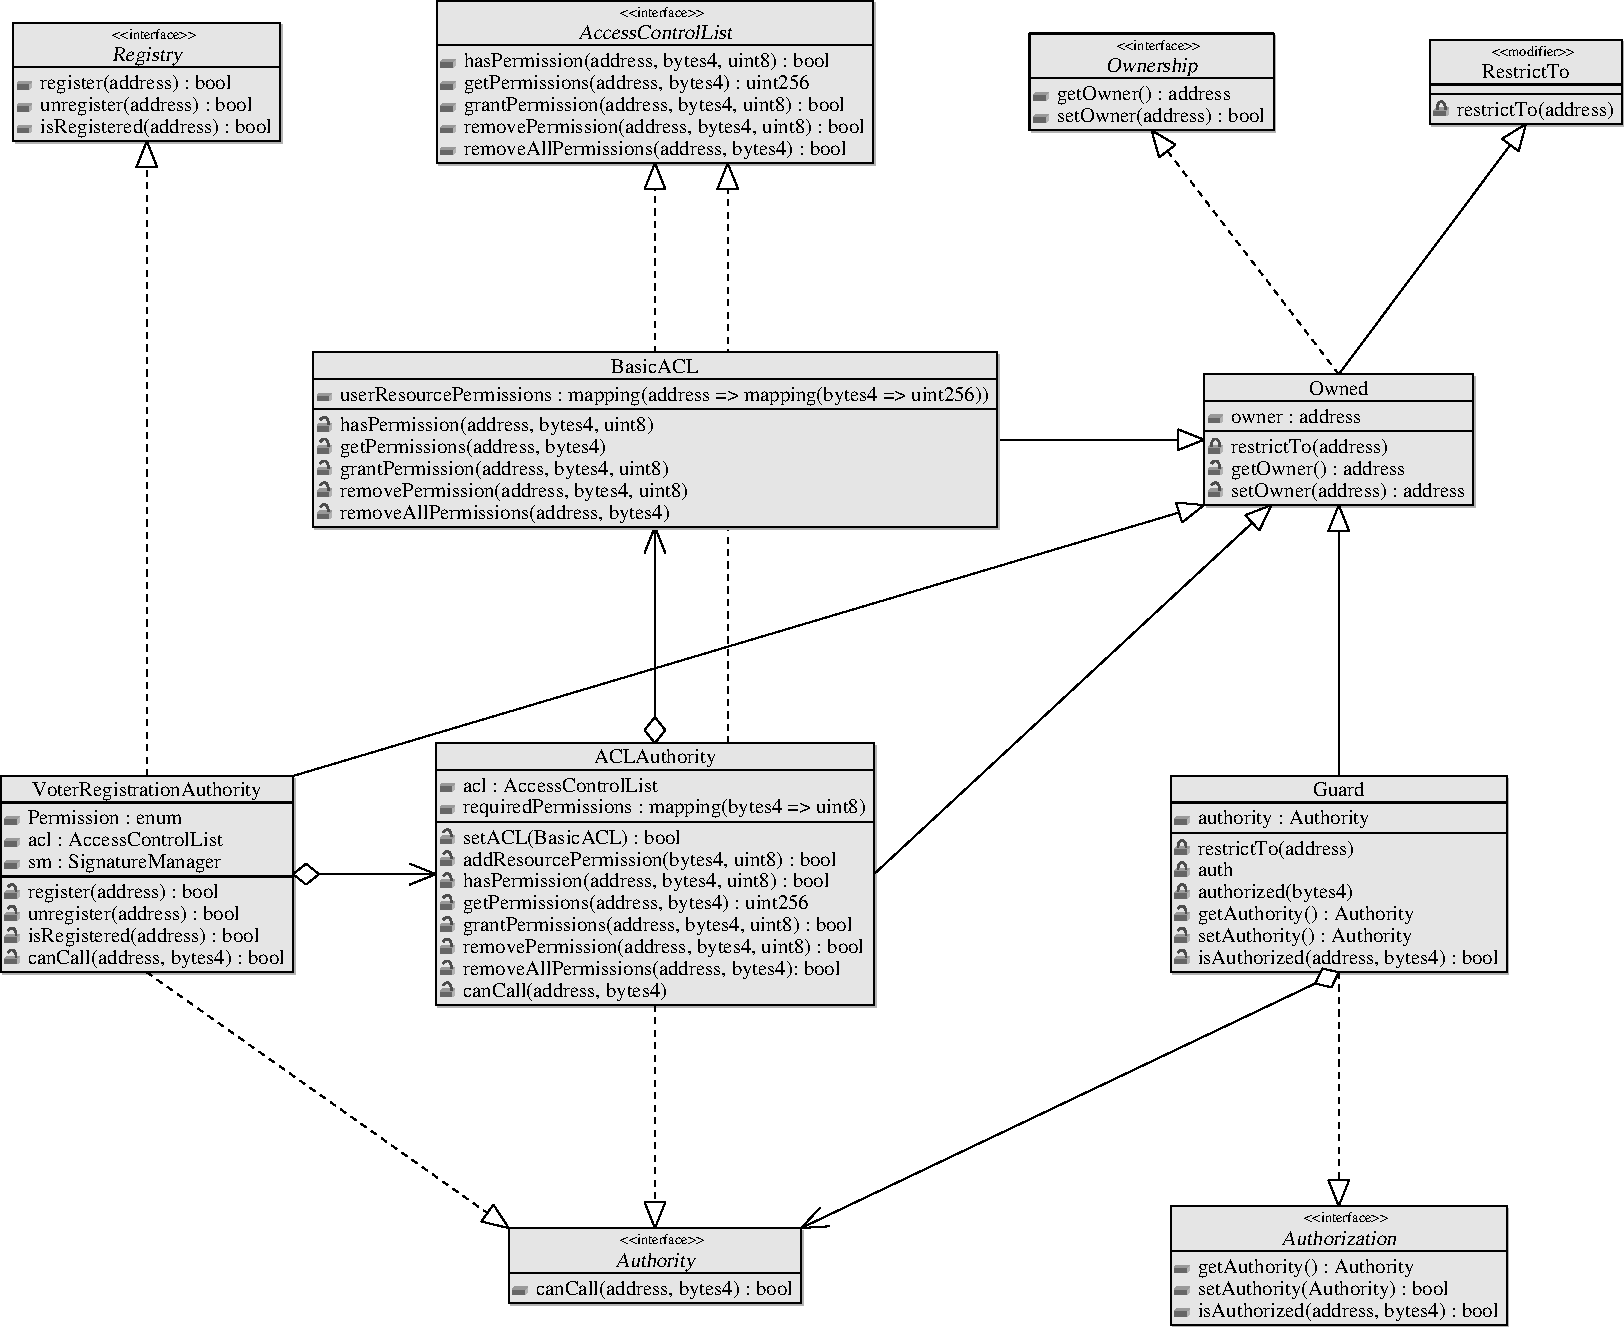
\includegraphics[width=\textwidth]{figures/authorization/figure}
  % \includestandalone[width=\textwidth]{\fig{authorization}}
  \caption{Authorization dependency graph modeling.}\label{fig:authorization}
\end{figure}

We define the \sol{Authorization} interface which offers mechanisms for
interacting with an \sol{Authority}. This interface defines \sol{getAuthority},
\sol{setAuthority}, and most importantly, \sol{isAuthorized}. A contract that
realizes the \sol{Authorization} interface is expected to aggregate an
\sol{Authority} but does not necessarily need one externally; for example, a
contract that provides \sol{Authorization} may also be its own \sol{Authority}.
Likewise, an \sol{Authority} can provide its own \sol{Authorization}. The
\sol{Authority} and \sol{Authorization} interfaces together form our access
control primitives.

The \sol{Guard} contract realizes the \sol{Authorization} interface and provides
the modifier functions \sol{auth} and \sol{authorized}. These can be applied to
other functions to easily restrict function-call access to accounts that the
\sol{Authority} has approved, e.g.,

\begin{solidity}[Guard Usage Example]
function sensitive () public auth returns (bool _success) {
  // The `auth` modifier prevents this function from being
  // called until the Authority has confirmed that the
  // the message sender has the proper privileges.
  return true;
}
\end{solidity}

This implementation conforms to a number of design principles: separation of
concerns, dependency inversion principle, open/closed principle, interface
segregation, substitution principle, and single responsibility principle.
Ultimately it provides the flexibility and resiliency necessary to build out a
wide variety of electoral systems.

\paragraph{Ownership}
Access control often starts before our \sol{Authority} and \sol{Authorization}
realizations. Most contracts offer a primitive form of access control through
\sol{Ownership}. All contracts and most contract functions are open and public
by design; thus, it is important to lock down sensitive contract functions from
deployment. A common pattern is to store the \solt{address} of the creator of a
contract as an owner in the contract state and to use that address to restrict
access to sensitive public-facing functions. More complicated ownership
mechanisms can be built using this pattern by leveraging contracts which
delegate ownership to another contract which can then define more complex access
control and management mechanisms. To facilitate in this and many other useful
patterns we introduce a simple \sol{Ownership} interface. The \sol{Ownership}
interface defines functions \sol{getOwner} and \sol{setOwner} which get and set
the account address of a contract's owners respectively.

To facilitate in restricting access of functions to a single account we also
define a contract \sol{RestrictTo} that provides a modifier function
\sol{restrictTo}. The \sol{restrictTo} modifier can be applied to any other
function and takes an account address argument; if the address of the account
calling a \sol{restrictTo} modified function does not match the argument
provided to \sol{restrictTo} (often the owner), then the function will
immediately exit and revert any changes to the contract. Finally, we realize and
extend these two contracts to form the concrete \sol{Owned} contract. This
pattern is so ubiquitous that most, if not all, concrete contracts in our
governance ecosystem will extend this contract.

\paragraph{Authority}
We need to provide access control beyond interfaces, standards, and single
account address restrictions. Our access control implementation leans towards
access control lists as a primitive that can be extended to provide other access
control mechanisms such as role-based access control. Alternatively, a contract
can realize the \sol{Authority} interface itself if ACLs are not a useful
abstraction.

\subparagraph{Access Control List}
We first define an ACL interface, \sol{AccessControlList}, which defines basic
ACL functionality: \sol{hasPermission}, \sol{getPermissions},
\sol{grantPermission}, \sol{removePermission}, and \sol{removeAllPermissions}.
The design supports assigning up to 256 unique permissions per contract
signature.

\subparagraph{Basic ACL}
Next we realize a concrete implementation of the \sol{AccessControlList}
interface named \sol{BasicACL}. \sol{BasicACL} is primarily a
database contract which creates a mapping from account address to a mapping of
functions (the first 4 bytes of their signature) to an unsigned 256-bit integer
that represents the permissions. This implementation is similar to what can be
found in POSIX compliant operating systems. In Java one might represent this
access control model as \codet{HashMap<Account, HashMap<Function,Permission>>}.

Naturally \sol{BasicACL} provides implementations for the functions defined by
\sol{AccessControlList}: \sol{hasPermission}, \sol{getPermissions},
\sol{grantPermission}, \sol{removePermission}, and \sol{removeAllPermissions}.
These work using bitwise NOT, OR, and AND operations to modify the 256-bit
unsigned integer representing permissions for a particular (account, function)
pair.

\subparagraph{ACL Authority}
We can easily build an \sol{ACLAuthority} out of our \sol{BasicACL} using the
adapter pattern and aggregation. We simply aggregate an instance of a
\sol{BasicACL} and realize the \sol{Authority} and \sol{AccessControlList}
interfaces. Finally, we lean on the \sol{hasPermission} function to implement
our \sol{canCall} function which presumably forwards our request to a
\sol{BasicACL} instance and returns the result. This structure also allows us to
implement a composite pattern and aggregate many trusted authorities into one.

\subparagraph{Voter Registration Authority}
Our final step is to use a facade to hide the more complex implementation
details from outside contracts. We introduce a \sol{VoterRegistrationAuthority}
which realizes the \sol{Registry} and \sol{Authority} interfaces.
The \sol{Registry} interface provides some nice abstractions:
\sol{register}, \sol{unregister}, and \sol{isRegistered}. We
presume the contract aggregates some number of \sol{AccessControlList}s as
a foundation for its \sol{Registry} function implementations, but does not
need to necessarily. Finally, the \sol{canCall} function leans on the
\sol{Registry} functions, specifically \sol{isRegistered} to grant
access to functions.

The end result is a clean, public, and composable voter registration authority.
